\documentclass[twocolumn, groupedaddress]{revtex4-1}
\usepackage[utf8]{inputenc}
\usepackage{amsmath}
\usepackage{amsfonts}
\usepackage{amssymb}
\usepackage{graphicx}											% Use pdf, png, jpg, or eps§ with pdflatex; use eps in DVI
\usepackage[left=2cm, right=2cm, top=2cm, bottom=2cm]{geometry}
\usepackage{float}												% for controlling the position of objects ie. tables

\usepackage{breqn}

\usepackage[small, bf]{caption}									%Adjust caption size of figures, tables, pictures...
\setlength{\captionmargin}{15pt}
										
\graphicspath{{images/}}											% folder where images are stored in current directory

% --------------------------- Code for placing two figure side by side ------------------------------------------------------------------
\usepackage{caption}
\usepackage{subcaption}

% --------------------------- Code for the bibliography ---------------------------------------------------------------------------------
\usepackage{natbib}												% For fancy in-text citations
\bibliographystyle{plain}



\begin{document}

\author{Curtis Rau}
\author{Benjamin Brophy}
\affiliation{Michigan State University}
\title{Computational Physics Project 2}

\begin{abstract}
In this project we saught to solve the Schr\"{o}dinger Equation for two interacting electrons in a cylindrically symmetric harmonic oscillator potential.  Potentials of this form are useful for simulating quantum dots.  Of particular interest are the low lying energy levels for this system which only have known analytical solutions for a few special cases \cite{taut}.  This paper gives an overview of the process of boiling down the Schrodinger equation to an ealily solvable one dimentional differential equation.  Then the method of discretizing the differential equation, and translating it into a matrix equation is discussed.  The Jacobi Method is introduced as the way in which the eigenvalues were obtained.  The Householder Algorithm was used to check the results from Jacobi's Method and both methods were in excellent agreement.
\end{abstract}

\maketitle


\section{Introduction}
In this project we aim to solve Schr\"{o}dinger's equation for two electrons in a three dimensional harmonic oscillator well with and without a repulsive Coulomb interaction, assuming that the move in a three dimensional harmonic oscillator potential. Here we have the Schr\"odinger for two electrons at $r_1$ and $r_2$ in such a potential

\begin{align}
[- \frac{\hbar^2}{2m} \left( \nabla_1^2 + \nabla_2^2 \right)				\nonumber
		+ \frac{1}{2}m\omega^2 \left( r_1^2 + r_2^2 \right)				\\
		+ \frac{ke^2}{|r_1^2-r_2^2|}
		]
		\psi (r_1,r_2)  = E \psi (r_1,r_2)
\end{align}


The Schr\"{o}dinger equation can be transformed to the radial equation in center of mass frame, where r represents the distance between electrons, and R is the position of the center of mass.

\begin{align}
  [ \left( - \frac{\hbar^2}{m} \frac{1}{r^2} \partial_r r^2 \partial_r + \frac{1}{4} m \omega^2 r^2 + \frac{k e^2}{r} \right) 	\nonumber \\
+ \left( - \frac{\hbar^2}{4m} \frac{1}{R^2} \partial_R R^2 \partial_R + m\omega^2 R^2 + \frac{\hbar l(l+1)}{R^2} \right) ]		\nonumber \\
 \psi (r) \theta (R) = (E_r + E_R) \psi (r) \theta (R)
\end{align}

We are only interested in the radial solution

\begin{equation}
\left( - \frac{\hbar^2}{m} \frac{1}{r^2} \partial_r r^2 \partial_r + \frac{1}{4} m \omega^2 r^2 + \frac{k e^2}{r} \right) \psi (r)  = E_r \psi (r)
\end{equation}

We can make the equation dimensionless which gives

\begin{equation}
\left( - \partial_\rho^2 + \rho^2 + \frac{\beta}{\rho} \right) u ( \rho ) = \lambda u(\rho ) \\
\left( - \partial_\rho^2 + V (\rho ) \right) u ( \rho ) = \lambda u(\rho )
\end{equation}

\section{Methods}

We discretize the equation as follows, where b and a are the end points of our model using N internal points. (There are N+2 total including end points)

\begin{equation}
\begin{aligned}
u(\rho) \to u(\rho_i) = u_i \\
\rho \to \rho_i = \rho_0 + i h \\
h = \frac{b-a}{n+1} \\
a = 0
\end{aligned}
\end{equation}

And use the following expression as an approximation of the second derivative:

$$u''=\frac{u(\rho+h)-2u(\rho)+u(\rho-h)}{h^2}$$

We can approximate the Schr\"odinger equation as 

$$\frac{u_{i+1}-2u_i+u_{i-1}}{h^2}+V_iu_i=\lambda u(\rho_i)$$

In terms of matrices, we have

\begin{align}
\left( \begin{array}{cccc}
\frac{2}{h^2} + V_1  &    -\frac{1}{h^2}   &                &            0            \\
   -\frac{1}{h^2}    & \frac{2}{h^2} + V_2 & -\frac{1}{h^2} &                         \\
                     &                     &     \ddots     &                         \\
                     &                     &                &     -\frac{1}{h^2}      \\
         0           &                     & -\frac{1}{h^2} & \frac{2}{h^2} + V_{N-1}
\end{array} \right)
\left( \begin{array}{cccc}
 u_1  \\
 u_2  \\
\dots \\
      \\
      \\
u_{N} \\
\end{array} \right)									\nonumber \\
 = \lambda
\left( \begin{array}{cccc}
 u_1  \\
 u_2  \\
\dots \\
      \\
      \\
u_{N} \\
\end{array} \right)
\end{align}

We will call the NxN matrix $\hat{A}$. We will perform a Jacobi rotation on this matrix, represented by multiplying both sides by $S_{ij}^T$, which as an identity matrix except with $c=cos\theta$ in positions $i,i$ and $j,j$, $s=sin\theta$ at position $i,j$, and $-s$ at position $j,i$ for some angle $\theta$.

\begin{equation}
S_{ij}^T = 
\left( \begin{array}{ccccccc}
1 &       &       &       &       &     &        0 \\
	 &\ddots &     &       &       &     &              \\
	 &       &  c    & \dots&  s    &     &              \\
	 &       &\vdots &       & \vdots&     &              \\
	 &       &   -s  & \dots &   c   &     &              \\
	 &       &       &       &       &\ddots&             \\
0 &       &       &       &       &     &   1  \\
\end{array} \right)
\end{equation} 


Note that:
\begin{itemize}  
\item Eigenvalues unchanged under orthogonal transforms such as a Jacobi rotation.
\item Eigenvectors change, but the length is preserved.
\item Dot product between vectors is conserved
\end{itemize}

\begin{eqnarray}
\hat{A} x = \lambda x \\
S^T A x = \lambda S^T x \\
S^T A S (S^T x) = \lambda (S^T x)
\end{eqnarray}

The values in the new matrix $\hat{A'}=S_{ij}^T\hat{A}$ can be found with the following relations, where $s=sin\theta$ and $c=cos\theta$ for some $\theta$:

\begin{eqnarray}
\hat{A'}_{ii} = c^2\hat{A}_{ii} - 2sc\hat{A}_{ij} + s^2\hat{A}_{jj} \\
\hat{A'}_{jj} = s^2\hat{A}_{ii} + 2sc\hat{A}_{ij} + c^2\hat{A}_{jj} \\
\hat{A'}_{ij} = \hat{A'}_{ji} = (c^2 - s^2)\hat{A}_{ij} + sc(\hat{A}_{ii} - \hat{A'}_{jj} )  \\
\hat{A'}_{ik} = \hat{A'}_{ki} = c\hat{A}_{ik} - s\hat{A}_{jk}, k\not= i,j \\
\hat{A'}_{jk} = \hat{A'}_{kj} = s\hat{A}_{ik} - c\hat{A}_{jk}, k\not= i,j \\
\hat{A'}_{kl} = \hat{A}_{kl} ,  k,l\not= i, 
\end{eqnarray}



We performed a Jacobian eigenvalue algorithm on this matrix to find the approximate eigenvalues. If we minimize all of the off-diagonal elements with orthogonal transforms, which preserve eigenvalues, then the remaining diagonal gives us the approximate eigenvalues of the matrix. A Jacobi rotation is one such orthogonal transform.

In our method, we first identify the largest off-diagonal element $A_{i,j}$ to use as the "pivot" in the Jacobi Rotation. So, we find the angle of rotation such that $A_{i,j}$ becomes zero. We perform a Jacobi rotation of that angle on $\hat{A}$ and call the rotated matrix our new $\hat{A}$.

 We repeat this process until either the largest off-diagonal element has absolute value less than a certain tolerance, 0.01, or until a maximum number of iterations is reached.

After many iterations, the off diagonal elements are minimized while the diagonals elements approach eigenvalues. 


\section{Analysis}
	
	Our first goal is to find the three lowest eigenstates for the case with no electrostatic potential to four leading digits. We have a few ways to go about this, as seen in the following table. In the case of the Householder method, our answer only depends on how much we discretize our matrix, or what value of N we choose. In this case we need N = 300 in order to obtain the lowest 3 eigenvalues to 4 leading digits. This takes .25 seconds to calculate. 
	In our crafted Jacobian method, the answer depends on both N and our tolerance. As described in our methods, we applied a special Jacobian rotation until the off diagonal elements our reduced below a certain tolerance. In the case of N=100, although the Householder method will not be accurate to 4 digits, we can obtain four leading correct digits with a tolerance of 0.001.This only takes 0.25 seconds and 13200 iterations to calculate.
	In the case of N=200, we can obtain four leading correct digits with a tolerance of 0.01. This only takes 2.9 seconds and 44012 iterations to calculate.
	In the case N=300, even though with a high tolerance of 0.1 gives us the eigenvalues within 4 leading digits, this brute force method takes 12.2 seconds compared to the .25 seconds for the Householder method.
	The number of iterations increases about as the square of N.
	
	
	\begin{table*}[t]
		\centering
		\begin{tabular}{ r | l || c | c | r | c | c | c | c | c | c }
			Size of &           & Householder & Jacobi & Iterations of & Jacobi  & Householder &  Jacobi & Householder & Jacobi & Householder \\
			Matrix  & Tolerance &    Time     &  Time  & Jacobi Method &   E1    &      E1     &    E2   &      E2     &   E3   &      E3     \\
			\hline
			100     & 0.1       &    0.01     &   0.15 &      8684     & 3.00030 &   3.22937   & 6.96709 & 6.96536 & 10.9168 & 10.91526 \\
			"       & 0.01      &     "       &   0.20 &     10667     & 2.99924 &      "      & 6.96537 &    "    & 10.9153 & "\\
			"       & 0.001     &     "       &   0.21 &     12076     & 2.99923 &      "      & 6.96536 &    "    & 10.9153 &\\
			"       & 0.0001    &     "       &   0.25 &     13200     &    "    &      "      &         &    "    &         & \\
			200     & 0.1       &    0.1      &   2.5  &     36836     & 3.00228 &   2.99986   &         &    "    &         & \\
			"       & 0.01      &     "       &   2.9  &     44012     & 2.99981 &      "      &         &    "    &         & \\
			"       & 0.001     &     "       &   3.2  &     49387     &    "    &      "      &         &    "    &         & \\
			"       & 0.0001    &     "       &   3.6  &     53888     &    "    &      "      &         &    "    &         & \\
			300     & 0.1       &    0.38     &  12.2  &     85521     & 3.00024 &   3.00000   &         &    "    &         & \\
			500     &  "        &    2.9      &   114  &    246826     & 3.00047 &   3.00003   & 7.00098 &    "    & 11.0005 & \\
			\hline
			 & & & & Expected Value: & 3 & 3 & 7 & 7 & 11 & 11
			
		\end{tabular}
		\caption{rhoMax = 5.0 \label{table:relults}}
	\end{table*}
	
	
\begin{figure*}[t]
	\centering
	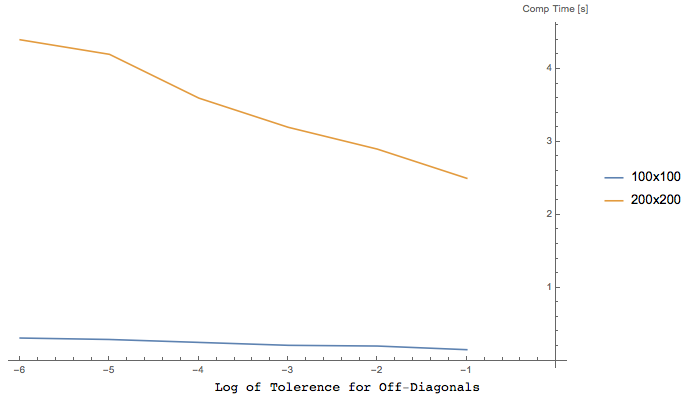
\includegraphics[width=.75\linewidth]{jacobiTimeDependence1}
	\caption{\label{fig:jacobiTimeDependence1} A plot of the Jacobi Method's time dependence on off diagonal element tolerence.  The plot legend gives the size of the matrix.}
\end{figure*}


\begin{figure*}[t]
	\centering
	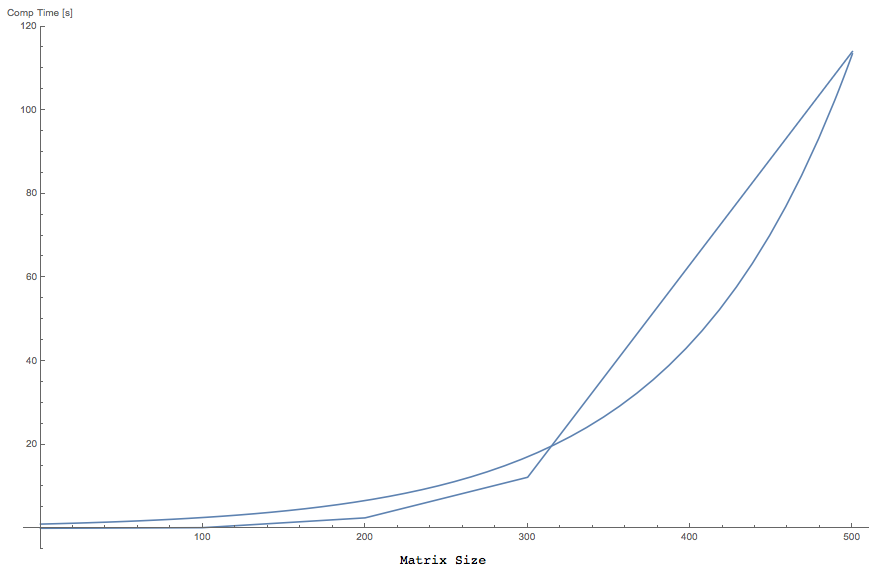
\includegraphics[width=.75\linewidth]{jacobiTimeDependence2}
	\caption{\label{fig:jacobiTimeDependence1} A plot of the Jacobi Method's time dependence on matrix size.  The best fit seemed to be exponential.}
\end{figure*}

\section{Conclusions}

\bibliography{project2Paper}

\end{document}
